\documentclass[11pt,letterpaper]{article}
\usepackage[margin=0.60in,top=0.58in,bottom=0.56in]{geometry}
\usepackage{mathptmx}
\usepackage{microtype}
\usepackage{graphicx}
\usepackage{booktabs}
\usepackage{array}
\usepackage{longtable}
\usepackage{amsmath,amssymb}
\usepackage[hidelinks]{hyperref}
\setlength{\parindent}{0pt}
\setlength{\parskip}{2.5pt}
\setlength{\columnsep}{0.25in}
\setcounter{secnumdepth}{0}
\renewcommand{\section}[1]{\vspace{3pt}\noindent\textbf{\underline{#1}}\par\vspace{1pt}}
\renewcommand{\subsection}[1]{\vspace{2pt}\noindent\textbf{#1}\par\vspace{1pt}}
\renewcommand{\familydefault}{\rmdefault}
\providecommand{\tightlist}{\setlength{\itemsep}{0pt}\setlength{\parskip}{0pt}}
\providecommand{\pandocbounded}[1]{\sbox0{#1}\ifdim\wd0>\linewidth\resizebox{\linewidth}{!}{#1}\else\usebox0\fi}
\title{\vspace{-1.2em}\textbf{\MakeUppercase{Neurologically Motivated
Self-Supervised Learning for Bilateral Gait Geometry}}\vspace{-0.5em}}
\author{\normalsize [Authors and affiliations to be inserted in the RISEx template]}
\date{}
\begin{document}
\twocolumn[
  \begin{@twocolumnfalse}
  \maketitle
  \vspace{-1.1em}
  \end{@twocolumnfalse}
]
\subsection{INTRODUCTION}\label{introduction}

AI systems that perceive people from video often compress articulated
motion into learned features. Before using such features in a
human-aware robotic pipeline, we should check whether they retain
task-relevant geometry. A horizontal reflection exchanges left and right
landmarks and reverses a signed contrast between their movement speeds.
This relation is relevant to gait asymmetry in stroke and Parkinson's
disease {[}1,2{]}, although our pose-derived contrast is neither a
diagnosis nor a clinical measurement. We test whether masked
joint-embedding predictive architecture (JEPA) training improves
recovery of this contrast.

\subsection{MATERIALS AND METHODS}\label{materials-and-methods}

We analyzed 625 quality-checked GAVD pose clips from 93 source videos
{[}3{]}. Clip-local preparation retains all 33 landmarks in a
64-by-33-by-3 sequence; four-frame patches form a 16-by-33 time-by-joint
grid. The encoder predicts hidden teacher features from visible tokens
{[}4{]}. Movement scores and affected-side labels are absent from
pretraining.

The score averages normalized left-minus-right median speeds for five
joint pairs. The null hypothesis was no improvement over the same
encoder at initialization. Five outer folds exclude whole source videos
from encoder and frozen ridge-readout fitting. Five seeds repeat matched
comparisons with shared starts, source draws, views, and updates. Scores
weight sources equally; intervals resample complete sources while
holding fitted models fixed.

\subsection{RESULTS AND DISCUSSION}\label{results-and-discussion}

\begin{figure}
\centering
\pandocbounded{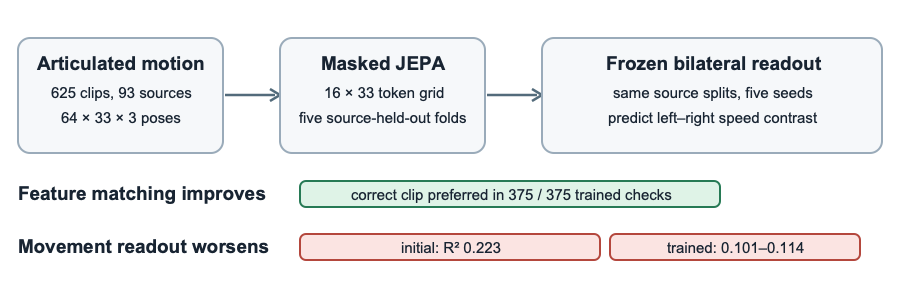
\includegraphics[keepaspectratio,alt={Study design and primary result.}]{risex_onepage_evidence.png}}
\caption{Study design and primary result.}
\end{figure}

{\def\LTcaptype{none} % do not increment counter
\begin{tabular}{@{}p{0.43\columnwidth}p{0.47\columnwidth}@{}}
\toprule\noalign{}
\begin{minipage}[b]{\linewidth}\raggedright
Prespecified check
\end{minipage} & \begin{minipage}[b]{\linewidth}\raggedright
Result
\end{minipage} \\
\midrule\noalign{}
Initial encoder, bilateral readout & \(R^2=0.223\) \\
Five trained teacher encoders & \(R^2=0.101\)--\(0.114\) \\
Trained minus matched initial & \(-0.109\) to \(-0.122\); each saved
interval below zero \\
Correct clip gives lower feature error & 375/375 trained checks; 33/75
at initialization \\
\end{tabular}
}

JEPA training made hidden features more specific to the correct clip,
yet trained encoders gave weaker bilateral-movement estimates. Motion
and connected-region masks showed no clear gain over matched random
references. This comparison tests latent correspondence against a known
geometric observable under a matched source-held-out control.

Feature errors use condition-specific teachers and can reflect pose,
viewpoint, or missing observations. The readout changes feature
dimension and adds motion and missingness summaries. Input preparation
changes the score (70.4\% sign agreement; \(R^2=0.218\)). These factors
may contribute to the deficit.

\subsection{CONCLUSIONS}\label{conclusions}

In this dataset and recipe, improved latent prediction did not improve
the frozen bilateral readout. Future human-aware robotics studies should
test future motion or interaction-relevant quantities with stable
targets and simple baselines.

\subsection{REFERENCES}\label{references}

{[}1{]} Patterson KK et al.~\emph{Arch Phys Med Rehabil} 89:304--310,
2008. {[}2{]} Lewek MD et al.~\emph{Gait Posture} 31:256--260, 2010.
{[}3{]} Ranjan R et al.~\emph{IEEE Access} 13:45321--45339, 2025.
{[}4{]} Assran M et al.~arXiv:2301.08243, 2023.
\end{document}
